%\documentclass{article}
\documentclass{chi2009}
\usepackage{times}
%\usepackage{uist}
\usepackage{url}
\usepackage{graphics}
\usepackage{color}

\begin{document}

% --- Copyright notice ---
\conferenceinfo{UIST'09}{October 4-7, 2008, Victoria, BC, Canada}
\CopyrightYear{2009}
\crdata{x-xxxxx-xxx-x/xx/xxxx}

% Uncomment the following line to hide the copyright notice
\toappear{}
% ------------------------

\bibliographystyle{plain}

\title{Exposing Disputed Statements on the Web}

%%
%% Note on formatting authors at different institutions, as shown below:
%% Change width arg (currently 7cm) to parbox commands as needed to
%% accommodate widest lines, taking care not to overflow the 17.8cm line width.
%% Add or delete parboxes for additional authors at different institutions. 
%% If additional authors won't fit in one row, you can add a "\\"  at the
%% end of a parbox's closing "}" to have the next parbox start a new row.
%% Be sure NOT to put any blank lines between parbox commands!
%%

\author{
\parbox[t]{9cm}{\centering
	     {\em Author Name removed for blind review}\\
}
\parbox[t]{9cm}{\centering
	     {\em Author Name removed for blind review}}
}

\maketitle

%RULE: Don't cite media reports unless I have to

\abstract
We present DisagreeWeb, a browser extension that aims to let users see when the information they are reading presents only one side of a disputed issue. As the user browses the web, DisagreeWeb highlights snippets of text that make claims that conflict with information on other web sites. If a user clicks on such a disputed claim then DisagreeWeb will show tem an argument graph showing the best evidence for and against the claim being true, as determined by other users of DisagreeWeb.

\keywords{CSCW, sensemaking, web, browsers, collaboration, mind mapping} 

\classification{H5.2 [Information interfaces and presentation]:
User Interfaces. - Graphical user interfaces.}

\terms{Design, Human Factors}

\keywords{Sense-making, Annotation, Argumentation, Web}


\tolerance=400 
  % makes some lines with lots of white space, but 	
  % tends to prevent words from sticking out in the margin

\section{INTRODUCTION}

The web provides users with a huge number of pages that they can read, but extracting accurate and balanced information from these pages can be difficult. Not everything on the web is accurate~\cite{Mintz2002,Neumann2003,Resnik98,Zhou2004} and many web sites have a strong political bias~\cite{Herman2002,Genzkow2007}. If a user is to form a rounded opinion about a topic then they will need to either stick to sources that they trust or spend time looking for evidence on other web sites that supports or opposes what they read. Even if a user tries hard to research every topic they read, they can still get caught out by beliefs that they had not realised were disputed.

In this paper we present DisagreeWeb, a tool helps users discover when information they read is disputed or presents only one side of a contentious issue. We hope that DisagreeWeb will make it easier for users to be be aware of points of view that contradict with those that they usually encounter.

When DisagreeWeb is used as a browser plugin it will highlight text on web pages that expresses or implies a disputed claim. If a user clicks on such a highlighted snippet then DisagreeWeb presents the user with a visualization of an argu

visualization that shows the user the best evidence for and against the claim, as judged by other users of DisagreeWeb.






that shows users when the information that they read conflicts with information available on other sources.

D

 DisagreeWeb is implemented as a browser extension 



aims to let users see when the information they are reading conflicts with information from other sources.

DisagreeWeb is implemented as a browser extension. 


The web suffers from filter failure~\cite{Shirky2008}. 



Part of the problem is that conventional web browsers present the web as a network of connected pages, when it is often the case that what the user is really interested in is the factual claims made by those pages, and the connections between those claims. While a web page will typically contain links to other articles, these typically only reference a small proportion of the other pages that discuss the topic, and are unlikely to include sources that disagree with the author. The best arguments supporting or opposing a claim may be distributed across a large number of disconnected pages, making it difficult for a user to assemble an argument from the pages on the web. The root of the problem is that the web is structured around where knowledge is coming from (pages written by particular authors) rather than what knowledge is about (the ideas contained on the pages). While this makes it easier for users to add knowledge to the web, it makes it hard for users to collate all the knowledge available on a topic.

\begin{figure}[tb]
	\begin{center}
	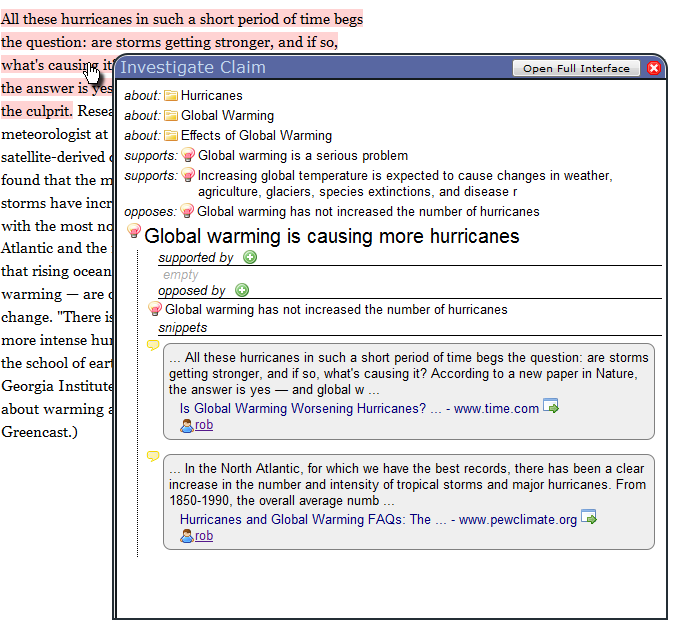
\includegraphics[width=6cm]{../screenshots/claim_popup_crop2.png}
	\caption{Click on a claim to investigate evidence for and against it}
	\label{claimview}
	\end{center}
\end{figure}

% \begin{figure}[tb]
% %	\begin{center}
%  	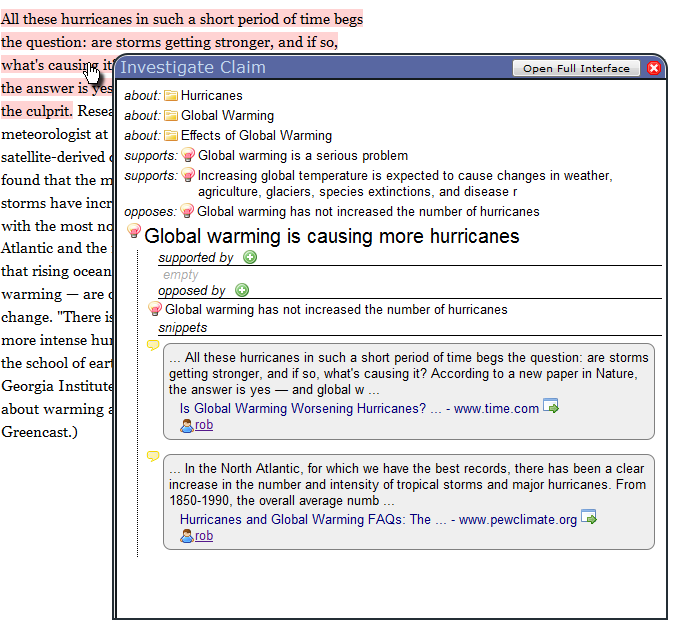
\includegraphics[width=6cm]{../screenshots/claim_popup_crop2.png}
%  	\caption{Click on a claim to investigate evidence for and against it}
%  	\label{claimview}
% 	\end{center}
% \end{figure}



\section{HIGHLIGHTING CONTROVERSIAL CLAIMS}

\section{CONNECTING UP THE ARGUMENT}

\section{THE THINK LINK SYSTEM}

\section{USER STUDIES}

\section{CONCLUSIONS}

\bibliographystyle{abbrv}
\bibliography{refs}

\end{document}



